\documentclass[11pt,a4paper]{article}

\usepackage[margin=2.5cm]{geometry}
\usepackage{booktabs}
\usepackage{xcolor}
\usepackage{graphicx}
\usepackage{float}
\usepackage{hyperref}
\usepackage{enumitem}
\usepackage{tikz}
\usepackage{pgfplots}
\pgfplotsset{compat=1.18}
\usetikzlibrary{arrows.meta,positioning}

\hypersetup{
    colorlinks=true,
    linkcolor=blue,
    urlcolor=blue
}

\title{Porting Milvus GPU Vector Search to AMD\\[0.3em]
\large HIP / hipVS / Knowhere on consumer RDNA3 (RX~7900~XTX)}
\author{Konstantin Kolchin}
\date{\today}

\begin{document}
\maketitle

\begin{abstract}
We describe a layered port of the Milvus GPU ANN path from NVIDIA cuVS/RAFT to
AMD hipVS/hipRAFT on ROCm, validated on a consumer RDNA3 GPU
(Radeon RX~7900~XTX, \texttt{gfx1100}).
The public HIP line is Milvus~\texttt{v2.5.4} + Knowhere~\texttt{2.5}
(\url{https://github.com/konkolchin/milvus-hip},
\url{https://github.com/konkolchin/knowhere-hip}),
with build/bench scripts in
\url{https://github.com/konkolchin/ann-harness-amd}.

\textbf{Correctness:} on peer-class GPUs (7900~XTX vs RTX~4080), sealed
\texttt{GPU\_IVF\_FLAT} and \texttt{GPU\_IVF\_PQ} recall@10 ladders match CUDA
on SIFT-1M and GIST-1M recipes used here.

\textbf{Speed (product path, batched Milvus QPS):}
\begin{itemize}[nosep,leftmargin=*]
  \item \textbf{SIFT-1M} is often stack-limited ($\sim$1$\times$ AMD/CUDA);
  \item \textbf{GIST-1M + IVF\_FLAT}: mostly peer / slight AMD lead
        (one mid-grid dip);
  \item \textbf{GIST-1M + IVF\_PQ} is GPU-heavier: AMD trails at roughly
        $0.60$--$0.80\times$ CUDA at matched recall.
\end{itemize}
Library microbenches (no Milvus): after an AMD-default
\texttt{blockDim}${=}512$ launch fix, hipVS \texttt{IVF\_PQ} ($m{=}32$) sits at
roughly $0.60$--$0.62\times$ cuVS mid-grid (was $\sim$0.5$\times$); GPU-heavy
\texttt{IVF\_FLAT} remains $\sim$1.3$\times$ --- useful context, not a product-QPS claim.
\end{abstract}

\tableofcontents
\clearpage

\section{Background}
\label{sec:background}

Milvus does not call cuVS from the Python client directly. The GPU stack is:

\begin{verbatim}
pymilvus / VectorDBBench
        |
   Milvus server
        |
   Knowhere  (CPU + GPU indexes)
        |
   GPU_IVF_FLAT / GPU_IVF_PQ / GPU_CAGRA / ...
        |
   NVIDIA: RAFT / cuVS
   AMD:    hipRAFT / hipVS   (ROCm-DS ports)
\end{verbatim}

\textbf{hipVS} aims at API compatibility with cuVS
(\url{https://github.com/ROCm-DS/hipVS}).
Stock Milvus CPU Docker images do not exercise the HIP path; GPU on AMD requires
a source build (or a custom image). NVIDIA GPU images do not run on AMD.

\section{Layered approach}
\label{sec:layers}

We did not replace cuVS inside Milvus in one step. Work proceeded in layers with
explicit pass gates:

\begin{table}[H]
\centering
\caption{Layer gates (lab host \texttt{amd-rx7900xtx}, ROCm~7.0.2)}
\label{tab:layers}
\begin{tabular}{@{}clp{0.52\textwidth}@{}}
\toprule
\textbf{\#} & \textbf{Focus} & \textbf{Pass evidence (summary)} \\
\midrule
0 & ROCm + CPU Milvus & \texttt{gfx1100} visible; CPU Standalone healthy \\
1 & hipRAFT / hipVS & Build; focused neighbors tests \\
1.5 & IVF packer on RDNA3 & Float IVF gtests 98/98 after
      \texttt{kIndexGroupSize}${=}32$ (warp32) \\
2 & Knowhere + HIP & Catch2 GPU L2 search gate green \\
3 & Milvus source & Sealed \texttt{GPU\_IVF\_*} build/load on HIP \\
4 & Fair benches & SIFT/GIST recall match vs CUDA; QPS plots below \\
\bottomrule
\end{tabular}
\end{table}

\noindent Detailed lab commands live in the harness README and the optional long
runbook \texttt{docs/porting\_milvus\_gpu\_to\_amd\_lab\_runbook.tex}.

\section{Hardware and fair compare}
\label{sec:fair}

\begin{itemize}[leftmargin=*]
  \item \textbf{AMD:} RX~7900~XTX (\texttt{gfx1100}), HIP Milvus Standalone,
        hide iGPU (\texttt{ROCR\_VISIBLE\_DEVICES=0}).
  \item \textbf{NVIDIA:} RTX~4080, \texttt{milvusdb/milvus:v2.5.4-gpu} Docker,
        same client scripts.
  \item \textbf{Client:} \texttt{scripts/run\_milvus\_hdf5.py} --- sealed index
        (\texttt{--flush}), batched search, report recall@10 and QPS.
  \item Peer-class boards ($\sim$320--355\,W TDP class), \emph{not} identical silicon.
        Use recall for port correctness; QPS for hardware/stack speed only.
\end{itemize}

Speed-up in figures $=$ AMD QPS / CUDA QPS.

\section{Results: QPS vs \texttt{nprobe}}
\label{sec:results}

Four product-path cases (HIP vs CUDA). Older appendix-style QPS/recall tables are
folded into these plots. Recall@10 matched between GPUs on every filled case
(see captions).

\subsection{SIFT-1M --- \texttt{GPU\_IVF\_FLAT}}
\label{sec:sift-flat}

\begin{figure}[H]
\centering
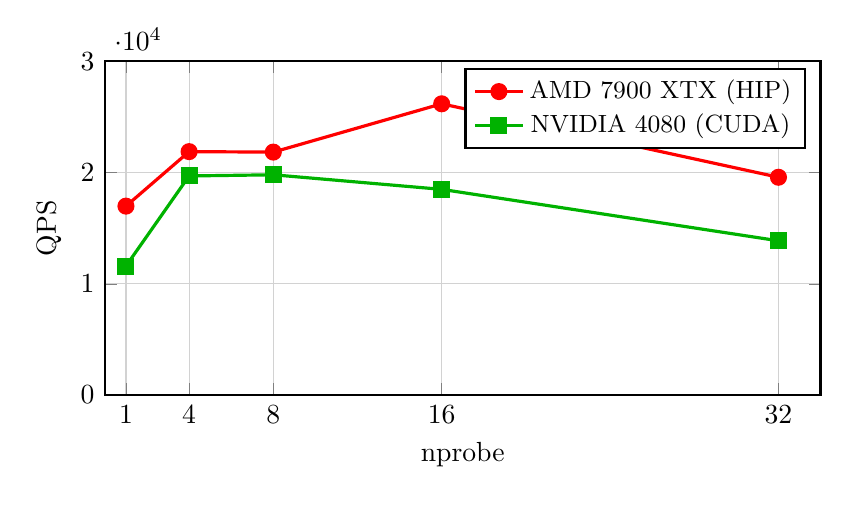
\begin{tikzpicture}
\begin{axis}[
  width=0.88\textwidth,
  height=0.48\textwidth,
  xlabel={nprobe},
  ylabel={QPS},
  xmin=0, xmax=34,
  ymin=0, ymax=30000,
  xtick={1,4,8,16,32},
  grid=both,
  major grid style={gray!35},
  legend style={at={(0.98,0.98)}, anchor=north east, font=\small},
  thick,
]
\addplot[red, mark=*, mark size=2.5pt, line width=1.15pt] coordinates {
  (1,16982) (4,21882) (8,21838) (16,26181) (32,19578)
};
\addlegendentry{AMD 7900 XTX (HIP)}
\addplot[green!70!black, mark=square*, mark size=2.5pt, line width=1.15pt] coordinates {
  (1,11597) (4,19695) (8,19800) (16,18490) (32,13868)
};
\addlegendentry{NVIDIA 4080 (CUDA)}
\end{axis}
\end{tikzpicture}
\caption{SIFT-1M, sealed \texttt{GPU\_IVF\_FLAT}, $nlist{=}1024$, $k{=}10$.
Recall@10 identical ($0.38\rightarrow0.98$).
AMD/CUDA QPS $\approx 1.1$--$1.5\times$ (stack-friendly recipe).}
\label{fig:sift-flat}
\end{figure}

\subsection{SIFT-1M --- \texttt{GPU\_IVF\_PQ} ($m{=}32$)}
\label{sec:sift-pq}

\begin{figure}[H]
\centering
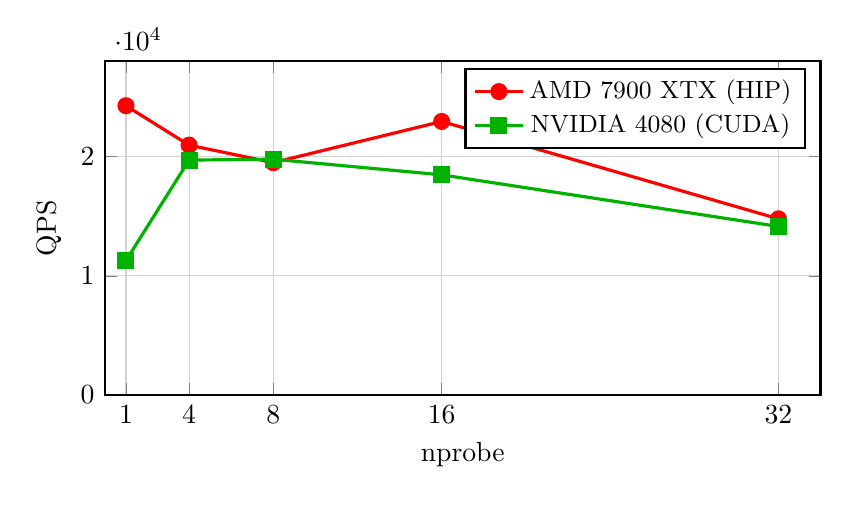
\begin{tikzpicture}
\begin{axis}[
  width=0.88\textwidth,
  height=0.48\textwidth,
  xlabel={nprobe},
  ylabel={QPS},
  xmin=0, xmax=34,
  ymin=0, ymax=28000,
  xtick={1,4,8,16,32},
  grid=both,
  major grid style={gray!35},
  legend style={at={(0.98,0.98)}, anchor=north east, font=\small},
  thick,
]
\addplot[red, mark=*, mark size=2.5pt, line width=1.15pt] coordinates {
  (1,24273) (4,20967) (8,19500) (16,22954) (32,14784)
};
\addlegendentry{AMD 7900 XTX (HIP)}
\addplot[green!70!black, mark=square*, mark size=2.5pt, line width=1.15pt] coordinates {
  (1,11282) (4,19714) (8,19786) (16,18475) (32,14144)
};
\addlegendentry{NVIDIA 4080 (CUDA)}
\end{axis}
\end{tikzpicture}
\caption{SIFT-1M, sealed \texttt{GPU\_IVF\_PQ} ($m{=}32$, $nbits{=}8$), $nlist{=}1024$, $k{=}10$.
Recall@10 identical ($0.36\rightarrow0.73$).
Mid/high \texttt{nprobe} $\approx 1\times$ AMD/CUDA --- still stack-limited vs library PQ.}
\label{fig:sift-pq}
\end{figure}

\subsection{GIST-1M --- \texttt{GPU\_IVF\_FLAT}}
\label{sec:gist-flat}

\begin{figure}[H]
\centering
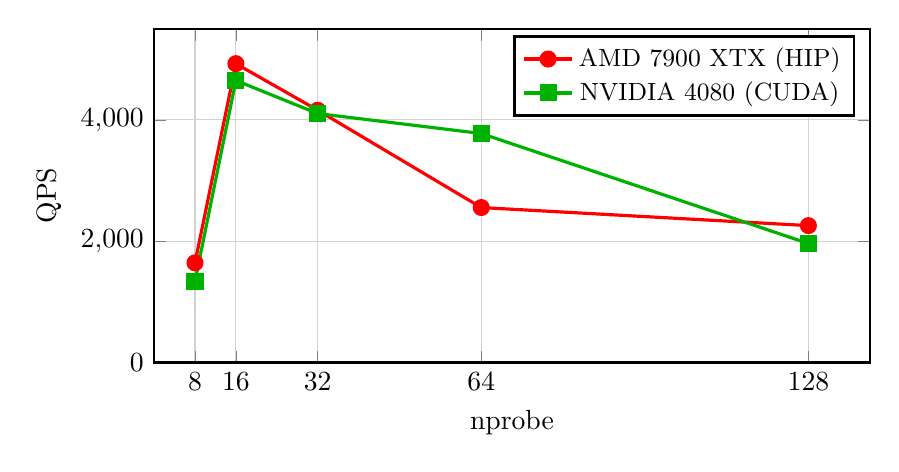
\begin{tikzpicture}
\begin{axis}[
  width=0.88\textwidth,
  height=0.48\textwidth,
  xlabel={nprobe},
  ylabel={QPS},
  xmin=0, xmax=140,
  ymin=0, ymax=5500,
  xtick={8,16,32,64,128},
  grid=both,
  major grid style={gray!35},
  legend style={at={(0.98,0.98)}, anchor=north east, font=\small},
  thick,
]
\addplot[red, mark=*, mark size=2.5pt, line width=1.15pt] coordinates {
  (8,1643) (16,4925) (32,4158) (64,2554) (128,2256)
};
\addlegendentry{AMD 7900 XTX (HIP)}
\addplot[green!70!black, mark=square*, mark size=2.5pt, line width=1.15pt] coordinates {
  (8,1339) (16,4648) (32,4103) (64,3774) (128,1961)
};
\addlegendentry{NVIDIA 4080 (CUDA)}
\end{axis}
\end{tikzpicture}
\caption{GIST-1M (960-d), sealed \texttt{GPU\_IVF\_FLAT}, $nlist{=}1024$, $k{=}10$
(2026-08-14).
Recall@10 matches ($\approx0.64\rightarrow0.99$).
AMD/CUDA QPS mostly $\sim$1.0--1.2$\times$ (exception: $0.68\times$ at \texttt{nprobe}=64).
First point is cold on both GPUs.
Sources: \texttt{results/milvus\_gist\_flat/FILLED.md}.}
\label{fig:gist-flat}
\end{figure}

\subsection{GIST-1M --- \texttt{GPU\_IVF\_PQ} ($m{=}32$)}
\label{sec:gist-pq}

\begin{figure}[H]
\centering
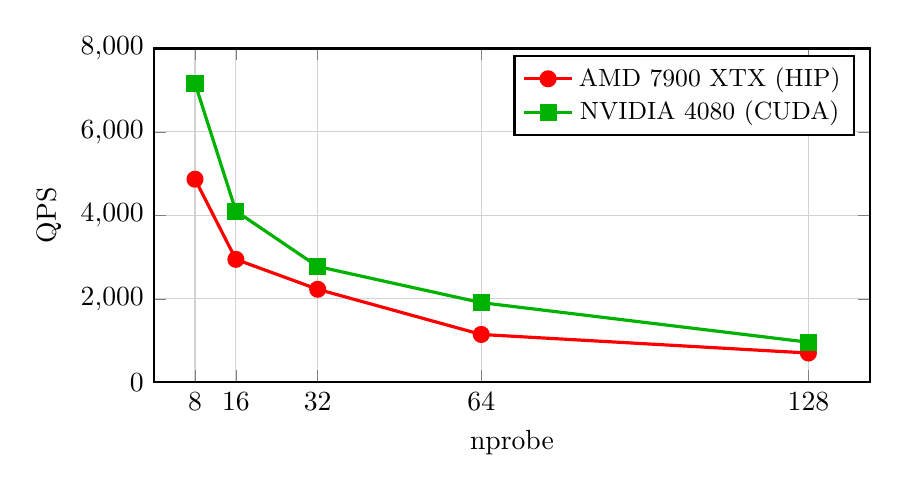
\begin{tikzpicture}
\begin{axis}[
  width=0.88\textwidth,
  height=0.48\textwidth,
  xlabel={nprobe},
  ylabel={QPS},
  xmin=0, xmax=140,
  ymin=0, ymax=8000,
  xtick={8,16,32,64,128},
  grid=both,
  major grid style={gray!35},
  legend style={at={(0.98,0.98)}, anchor=north east, font=\small},
  thick,
]
\addplot[red, mark=*, mark size=2.5pt, line width=1.15pt] coordinates {
  (8,4867) (16,2945) (32,2228) (64,1145) (128,700)
};
\addlegendentry{AMD 7900 XTX (HIP)}
\addplot[green!70!black, mark=square*, mark size=2.5pt, line width=1.15pt] coordinates {
  (8,7167) (16,4102) (32,2774) (64,1908) (128,959)
};
\addlegendentry{NVIDIA 4080 (CUDA)}
\end{axis}
\end{tikzpicture}
\caption{GIST-1M (960-d), sealed \texttt{GPU\_IVF\_PQ} ($m{=}32$, $nbits{=}8$),
$nlist{=}1024$, $k{=}10$ (2026-07-28).
Recall@10 matches ($\approx0.25\rightarrow0.27$; PQ tax on 960-d, not a wrong port).
AMD/CUDA QPS $\approx 0.60$--$0.80\times$ --- fair GPU-heavy product-path speed signal.
Sources: \texttt{results/milvus\_gist\_pq/FILLED.md}.}
\label{fig:gist-pq}
\end{figure}

\section{How to read the four plots}
\label{sec:read}

\begin{itemize}[leftmargin=*]
  \item \textbf{Recall match} on FLAT and PQ $\Rightarrow$ the HIP port returns the
        same answer quality as CUDA on these recipes.
  \item \textbf{SIFT} (Figures~\ref{fig:sift-flat},~\ref{fig:sift-pq}): absolute
        Milvus QPS is far below direct hipVS/cuVS library rates; AMD$\approx$CUDA is a
        \emph{stack-overhead} verdict, not an ANN-kernel parity claim.
  \item \textbf{GIST FLAT} (Figure~\ref{fig:gist-flat}): high recall ladder;
        QPS mostly peer / slight AMD lead (one mid-grid dip).
  \item \textbf{GIST PQ} (Figure~\ref{fig:gist-pq}): GPU work dominates; NVIDIA ahead
        at matched recall --- the honest product-path speed gap for this PoC.
  \item \textbf{Library context} (optional microbench, no Milvus;
        Figures~\ref{fig:lib-pq-bt512},~\ref{fig:lib-pq}):
        AMD-default \texttt{blockDim}${=}512$ lifts hipVS PQ $\sim$+25\% vs stock
        on the same GPU; vs cuVS the mid-grid ratio is $\sim$0.60--0.62$\times$
        (was $\sim$0.48--0.50$\times$). GPU-heavy \texttt{IVF\_FLAT} $\sim$1.3$\times$
        (\texttt{results/lib\_bench/}).
\end{itemize}

\section{Library PQ: AMD launch default (\texttt{blockDim}${=}512$)}
\label{sec:lib-bt512}

Stock hipVS \texttt{compute\_similarity\_select} auto-shrinks block size with an
NVIDIA-oriented occupancy heuristic. On \texttt{gfx1100}, preferring
\texttt{blockDim}${=}512$ raised library IVF-PQ search QPS by $\sim$25--35\%
at matched recall (Table~\ref{tab:lib-bt512-delta};
harness A/B: \texttt{results/lib\_bench/LAUNCH\_KNOBS.md}).
That preference is now the AMD default in our hipVS line
(\url{https://github.com/konkolchin/hipVS}, commit \texttt{aae4bbe};
harness patch \texttt{0006}). A separate score-loop micro-opt (pipeline / pq8)
was tried and \textbf{reverted} --- no QPS win.

\begin{table}[H]
\centering
\caption{Library hipVS \texttt{IVF\_PQ} $m{=}32$ on RX~7900~XTX:
July stock vs AMD-default \texttt{blockDim}${=}512$ (same recipe; recall matched).}
\label{tab:lib-bt512-delta}
\begin{tabular}{@{}rrrrr@{}}
\toprule
\textbf{nprobe} & \textbf{Stock QPS} & \textbf{bt512 QPS} & \textbf{$\Delta$} & \textbf{vs cuVS (bt512)} \\
\midrule
8  & 710{,}989  & 862{,}599  & $+21\%$ & $0.61\times$ \\
16 & 393{,}742  & 497{,}091  & $+26\%$ & $0.62\times$ \\
32 & 217{,}275  & 269{,}845  & $+24\%$ & $0.60\times$ \\
\bottomrule
\end{tabular}
\end{table}

\begin{figure}[H]
\centering
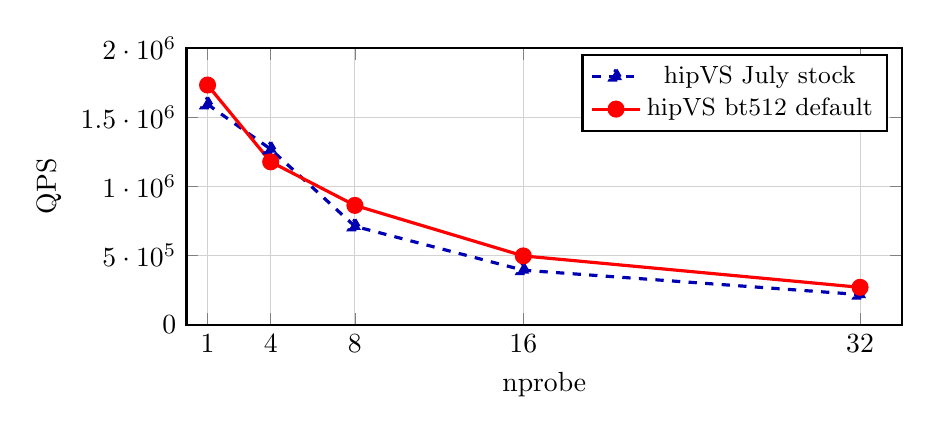
\begin{tikzpicture}
\begin{axis}[
  width=0.88\textwidth,
  height=0.42\textwidth,
  xlabel={nprobe},
  ylabel={QPS},
  xmin=0, xmax=34,
  ymin=0, ymax=2.0e6,
  xtick={1,4,8,16,32},
  grid=both,
  major grid style={gray!35},
  legend style={at={(0.98,0.98)}, anchor=north east, font=\small},
  thick,
  scaled ticks=false,
]
% Only the two hipVS series --- y-scale matches AMD rates so +25% is visible.
\addplot[blue!70!black, mark=triangle*, mark size=2.5pt, line width=1.15pt, dashed] coordinates {
  (1,1593707) (4,1268942) (8,710989) (16,393742) (32,217275)
};
\addlegendentry{hipVS July stock}
\addplot[red, mark=*, mark size=2.5pt, line width=1.15pt] coordinates {
  (1,1733219) (4,1177594) (8,862599) (16,497091) (32,269845)
};
\addlegendentry{hipVS bt512 default}
\end{axis}
\end{tikzpicture}
\caption{Same GPU, same library API: stock launch heuristic vs AMD-default
\texttt{blockDim}${=}512$. Mid-grid lift $\sim$+21--26\% (Table~\ref{tab:lib-bt512-delta}).
Y-axis is scaled to hipVS only --- do not compare to cuVS on this plot.}
\label{fig:lib-pq-bt512}
\end{figure}

\begin{figure}[H]
\centering
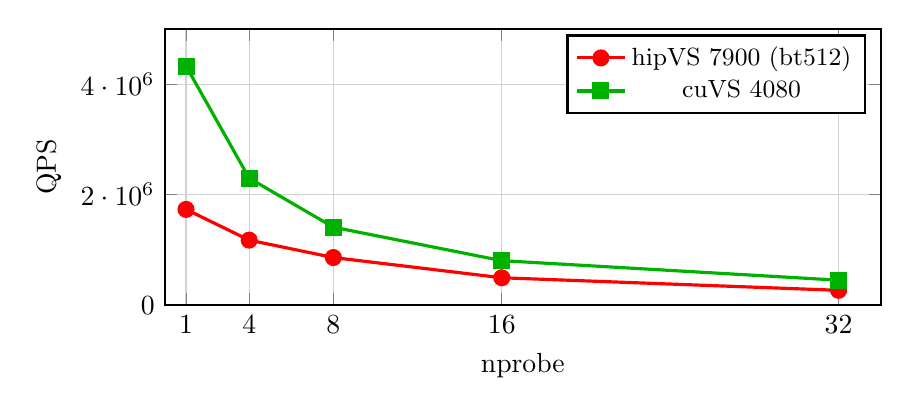
\begin{tikzpicture}
\begin{axis}[
  width=0.88\textwidth,
  height=0.42\textwidth,
  xlabel={nprobe},
  ylabel={QPS},
  xmin=0, xmax=34,
  ymin=0, ymax=5e6,
  xtick={1,4,8,16,32},
  grid=both,
  major grid style={gray!35},
  legend style={at={(0.98,0.98)}, anchor=north east, font=\small},
  thick,
  scaled ticks=false,
]
\addplot[red, mark=*, mark size=2.5pt, line width=1.15pt] coordinates {
  (1,1733219) (4,1177594) (8,862599) (16,497091) (32,269845)
};
\addlegendentry{hipVS 7900 (bt512)}
\addplot[green!70!black, mark=square*, mark size=2.5pt, line width=1.15pt] coordinates {
  (1,4326105) (4,2297667) (8,1411722) (16,806267) (32,453316)
};
\addlegendentry{cuVS 4080}
\end{axis}
\end{tikzpicture}
\caption{Remaining peer-GPU library gap after the launch fix:
hipVS/cuVS $\sim$0.60--0.62$\times$ mid-grid (was $\sim$0.48--0.50$\times$).
cuVS absolute QPS is much higher, so this axis dwarfs the hipVS-only delta
in Figure~\ref{fig:lib-pq-bt512}.}
\label{fig:lib-pq}
\end{figure}

\section{Public repositories}
\label{sec:repos}

\begin{table}[H]
\centering
\caption{Public HIP line (not upstream \texttt{master})}
\label{tab:repos}
\begin{tabular}{@{}llp{0.42\textwidth}@{}}
\toprule
\textbf{Piece} & \textbf{Repo} & \textbf{Pin} \\
\midrule
Milvus & \url{https://github.com/konkolchin/milvus-hip} & \texttt{v2.5.4} \\
Knowhere & \url{https://github.com/konkolchin/knowhere-hip} & \texttt{2.5} \\
Harness & \url{https://github.com/konkolchin/ann-harness-amd} & \texttt{master} \\
hipVS / hipRAFT & \url{https://github.com/konkolchin/hipVS} (+ ROCm-DS)
  & \texttt{release/rocmds-25.10} + gfx1100 patches (incl.\ bt512) \\
\bottomrule
\end{tabular}
\end{table}

\noindent Start from the Milvus README in that fork and the harness Layer~4 scripts
(\texttt{run\_milvus\_layer4*.sh}, \texttt{run\_milvus\_layer4\_gist\_*.sh}).

\section{Scope and limitations}
\label{sec:scope}

\begin{itemize}[leftmargin=*]
  \item Consumer RDNA3 PoC --- not a claim of full NVIDIA feature or speed parity.
  \item \texttt{GPU\_CAGRA}: unfiltered search only on \texttt{gfx1100}; filtered /
        bitset paths are out of scope for this release.
  \item Stock hipVS needed an RDNA3 IVF packer fix (\texttt{kIndexGroupSize}${=}32$
        with \texttt{USE\_WARPSIZE\_32}); see harness \texttt{patches/hipvs/}.
  \item PQ search launch: AMD-default \texttt{blockDim}${=}512$ is on
        (Section~\ref{sec:lib-bt512}); product Milvus must load the rebuilt
        \texttt{libcuvs} (restart Standalone; do not run Docker
        \texttt{milvus-standalone} alongside the HIP binary).
\end{itemize}

\section{References}
\label{sec:refs}

\begin{itemize}[leftmargin=*]
  \item Harness: \url{https://github.com/konkolchin/ann-harness-amd}
  \item Lab runbook (long form): \texttt{docs/porting\_milvus\_gpu\_to\_amd\_lab\_runbook.tex}
  \item hipVS: \url{https://github.com/ROCm-DS/hipVS}
  \item CUDA~4080 runbook: \texttt{docs/cuda\_4080\_benchmark\_runbook.md}
  \item GIST PQ filled: \texttt{results/milvus\_gist\_pq/FILLED.md}
  \item GIST FLAT filled: \texttt{results/milvus\_gist\_flat/FILLED.md}
  \item Library PQ / FLAT: \texttt{results/lib\_bench/FILLED\_pq\_m32.md},
        \texttt{FILLED\_flat\_heavy.md}
  \item PQ launch knobs / bt512 default: \texttt{results/lib\_bench/LAUNCH\_KNOBS.md}
  \item hipVS DXC fork (bt512): \url{https://github.com/konkolchin/hipVS}
\end{itemize}

\end{document}
